\chapter{ベクトルと行列と統計学}

本章では, これまで学んだベクトルや行列が, 統計学と融合して, 強力な道具になることを学ぶ。
なお, 本章では, 特に断らないときは, $i$, $j$, $k$, $l$, $m$, $n$, $N$を任意の自然数とする。

\section{行列の積と数ベクトルの内積}\label{sect:matrix_product_again}

\ref{chap:matrix}章で学んだように, 行列とは, 数が格子状に並んだものであり, 
縦の並びを「列」, 横の並びを「行」という。行列の第$i$行とは, 上から数えて
$i$番目の「横の並び」であり, 第$j$列とは, 左から数えて$j$番目の「縦の並び」
である。第$i$行と第$j$列の交差するところにある数を, その行列の$(i, j)$成分という。

本章では, 記述の簡略化のために, 行列$A$の$(i, j)$成分を, $[A]_{ij}$と書く
(この添字の$ij$は「$i$と$j$の積」ではない。$i$と$j$を並べて
書くことである)。例えば, 
\begin{eqnarray}
A=\begin{bmatrix}
1 & 2\\
3 & 4\\
\end{bmatrix}
\end{eqnarray}
のとき, $[A]_{11}=1$, $[A]_{12}=2$, $[A]_{21}=3$, $[A]_{22}=4$である。

さて, 2つの行列$A,\,B$について, $A$の列数(横幅)と$B$の行数(縦幅)
が等しいときに限り, 積$AB$を次のように定義する: 
\begin{eqnarray}
[AB]_{ij}:=\sum_{k=1}^{m}[A]_{ik}[B]_{kj}\label{eq:defmatrixproduct}
\end{eqnarray}
ここで, $m, n, l$は任意の自然数で, $n$は$A$の行数, $m$は$A$の列数かつ$B$の行数, 
$l$は$B$の列数とする。$i, k, j$はそれぞれ$m, n, l$以下の自然数である。
これは既に学んだことを書きなおしただけである。

\eref{eq:defmatrixproduct}を, $\sum$を使わないで書きなおすと, 
\begin{eqnarray}
[AB]_{ij}=[A]_{i1}[B]_{1j}+[A]_{i2}[B]_{2j}+\cdots+[A]_{im}[B]_{mj}\nonumber\\\label{eq:defmatrixproduct2}
\end{eqnarray}
となる。これは, 数ベクトルの内積と見ることができる。
\begin{eqnarray}
[AB]_{ij}=([A]_{i1}, [A]_{i2}, \cdots, [A]_{im})\bullet 
\begin{bmatrix}
[B]_{1j}\\
[B]_{2j}\\
\vdots\\
[B]_{mj}\\
\end{bmatrix}\quad\quad\quad\quad\quad\label{eq:defmatrixproduct3}
\end{eqnarray}
と書けるからだ。ここで, 
\begin{eqnarray*}
([A]_{i1}, [A]_{i2}, \cdots, [A]_{im})
\end{eqnarray*}
は, 行列$A$の第$i$行の行ベクトルであり, 
\begin{eqnarray*}
\begin{bmatrix}
[B]_{1j}\\
[B]_{2j}\\
\vdots\\
[B]_{mj}\\
\end{bmatrix}\end{eqnarray*}
は, 行列$B$の第$j$列の列ベクトルなので, \eref{eq:defmatrixproduct3}
は以下のように解釈できる: \textgt{行列$A, B$について, その積$AB$の$(i, j)$成分は, 
$A$の第$i$\textgt{行}ベクトルと$B$の第$j$\textgt{列}ベクトルの内積である。}

このことを念のため, 式でも書いておこう。$A$の第$i$\textgt{行}ベクトルを${\bf a}_i$, 
$B$の第$j$\textgt{列}ベクトルを${\bf b}_j$とすると, 
\begin{eqnarray}
AB=
\begin{bmatrix}
{\bf a}_1\bullet{\bf b}_1 & {\bf a}_1\bullet{\bf b}_2 & \cdots & {\bf a}_1\bullet{\bf b}_l\\
{\bf a}_2\bullet{\bf b}_1 & {\bf a}_2\bullet{\bf b}_2 & \cdots & {\bf a}_2\bullet{\bf b}_l\\
\vdots & \vdots & \ddots & \vdots\\
{\bf a}_n\bullet{\bf b}_1 & {\bf a}_n\bullet{\bf b}_2 & \cdots & {\bf a}_n\bullet{\bf b}_l\\
\end{bmatrix}\label{eq:AB_matprod_inprod}
\end{eqnarray}
このような考え方は, 後々, 大切になってくる。\\


\section{行列の積の結合法則}

これから行列に関する大切な定理を証明していく。その前にいくつか
準備をする。まず, 総和($\Sigma$)の添字は, はじめの値と終わりの値
($\Sigma$記号の上下に書かれるべき値)を省略することがある。例えば\eref{eq:defmatrixproduct}は, 
\begin{eqnarray*}
[AB]_{ij}:=\sum_{k}[A]_{ik}[B]_{kj}
\end{eqnarray*}
と書いてもよいことにする。このとき, $k$の動く範囲は$A$の列数(かつ$B$の行数)
全体である。このように, 可能な範囲全体を添字が動くときは, 
上記のような省略をする。\\

次に, 複数の添字による総和は, 順序を入れ替えてもOKであることを確認しておこう。例えば, 
2つの添字で表される量$a_{ij}$について, 
\begin{eqnarray*}
&&\sum_{i=1}^{3}\sum_{j=1}^{2}a_{ij}\\
&&\sum_{j=1}^{2}\sum_{i=1}^{3}a_{ij}
\end{eqnarray*}
という2つの式は同じである。なぜか? それぞれは
\begin{eqnarray*}
&&a_{11}+a_{12}+a_{21}+a_{22}+a_{31}+a_{32}\\
&&a_{11}+a_{21}+a_{31}+a_{12}+a_{22}+a_{32}
\end{eqnarray*}
となり, これらは足し算の順序が違うだけで, 本質的には同じである。
$i, j$の動く範囲がもっと大きくなってもそうなることは想像・理解
できるだろう。\\

さて, 話を戻す。いま, 3つの行列$A, B, C$を考える。$A$の列数=$B$の行数であり, 
$B$の列数=$C$の行数であるとする。このとき, 
\begin{eqnarray}(AB)C=A(BC)\label{eq:matrix_association_law}\end{eqnarray}
が成り立つ(定理)。証明は以下のとおり: $i$, $j$を自然数とする。\eref{eq:defmatrixproduct}より, 
\begin{eqnarray*}
[(AB)C]_{ij}&=&\sum_{l}[AB]_{il}[C]_{lj}\\
&=&\sum_{l}(\sum_{k}[A]_{ik}[B]_{kl})[C]_{lj}\\
&=&\sum_{l}\sum_{k}[A]_{ik}[B]_{kl}[C]_{lj}\\
&=&\sum_{k}\sum_{l}[A]_{ik}[B]_{kl}[C]_{lj}\\
&=&\sum_{k}[A]_{ik}\sum_{l}[B]_{kl}[C]_{lj}\\
&=&\sum_{k}[A]_{ik}[BC]_{kj}\\
&=&[A(BC)]_{ij}
\end{eqnarray*}
従って, $(AB)C=A(BC)$\qed
\mv

\eref{eq:matrix_association_law}を「行列の積の結合法則」という。
本章の後半では, この考え方が活躍する。

\begin{q}\label{q:invmatrix_product3} 行列の積の結合法則の
証明を再現せよ。
\end{q}
\mv

\section{逆行列}

\ref{chap:matrix}章で学んだように, 正方行列$A$について, ある正方行列$B$が, 
\begin{eqnarray}AB=BA=I\end{eqnarray}
となる場合($I$は単位行列), $B$は$A$の\underline{逆行列}\index{ぎゃくぎょうれつ@逆行列}である, 
と言って, $B=A^{-1}$と書く。すなわち, 
\begin{eqnarray}AA^{-1}=A^{-1}A=I\label{eq:matrix_inverse}\end{eqnarray}
である。全ての正方行列が逆行列を持つとは限らない。逆行列を持つ正方行列を\underline{正則行列}
\index{せいそくぎょうれつ@正則行列}と呼ぶ。

\begin{q}\label{q:invmatrix_product} $n$次正則行列$A, B$について, 次式を示せ:
\begin{eqnarray}(AB)^{-1}=B^{-1}A^{-1}\label{eq:ABinverse}\end{eqnarray}
\end{q}

次の節で, \eref{eq:ABinverse}に似た式が出てくる。それらは本章の後半で活躍する。\\
\mv

\section{転置行列}

行列$A$の行と列を入れ替えてできる
行列(右上と左下をひっくり返した行列)を, 「$A$の\underline{転置行列}
 \index{てんちぎょうれつ@転置行列}」とか, 縮めて「$A$の\underline{転置} 
\index{てんち@転置}」と呼び, $^{\text t}A$とか$A^{\text T}$とあらわす
\footnote{肩のtやTは, transpose (転置)の頭文字を意味する。}。すなわち, 
任意の(可能な)自然数$i, j$について, 
\begin{eqnarray}
[^{\text t}A]_{ij}:=[A]_{ji}\label{eq:def_transpose_component}
\end{eqnarray}
である。

\begin{exmpl}
\begin{eqnarray}
A=\begin{bmatrix}
1 & 2 & 3\\
4 & 5 & 6\\
7 & 8 & 9\\
\end{bmatrix}
\quad\text{ならば, }
^{\text t}A=\begin{bmatrix}
1 & 4 & 7\\
2 & 5 & 8\\
3 & 6 & 9\\
\end{bmatrix}
\quad\quad\quad\quad\label{eq:exmpl_matrix_A00}
\end{eqnarray}
である。(例おわり)\qed\end{exmpl}

当然ながら, 転置を2回行うと, もとの行列に戻る。すなわち, 任意の行列$A$について, 
次式が成り立つ:
\begin{eqnarray}
^{\text t}(^{\text t} A)=A
\end{eqnarray}
証明: 任意の(可能な)自然数$i, j$について, \eref{eq:def_transpose_component}より, 
$[^{\text t}(^{\text t} A)]_{ij}=[^{\text t} A]_{ji}=[A]_{ij}$, 従って, $[^{\text t}(^{\text t} A)]=A$\qed
\mv

また, 2つの行列$A, B$が足せるとき, 
\begin{eqnarray}
^{\text t}(A+B)=\,^{\text t}A+\,^{\text t}B
\end{eqnarray}
が成り立つ。証明: 任意の(可能な)自然数$i, j$について, \eref{eq:def_transpose_component}より, 
$[^{\text t}(A+B)]_{ij}=[A+B]_{ji}$。ところが, $[A+B]_{ji}=[A]_{ji}+[B]_{ji}$である
(行列の和の定義)。
従って, 
$[^{\text t}(A+B)]_{ij}=[A]_{ji}+[B]_{ji}=[^{\text t}A]_{ij}+[^{\text t}B]_{ij}$
$=[^{\text t}A+^{\text t}B]_{ij}$, 従って, 与式が成り立つ。\qed
\mv

数ベクトルも行列の一種とみなせるから, その転置を考えることができる:
\begin{exmpl}
\begin{eqnarray}
{\bf x}=
\begin{bmatrix}
2\\
1\\
-1\\
\end{bmatrix}\quad
\text{ならば, }\quad^{\text t}{\bf x}=(2, 1, -1)\label{eq:exmpl_matrix_x00}
\end{eqnarray}
{\small 注: 行ベクトルは, $(2,\,1,\,3)$のようにコンマでわけて書くこともあるし, 
$(2\,\,1\,\,3)$のように, 行列っぽく(コンマを入れないで)書くこともある。どちらでもよい。
また, 括弧は丸括弧()を使うことも角括弧$[]$を使うこともある。どちらでもよい。}
(例おわり)\qed\end{exmpl}

このように, 列ベクトルの転置は行ベクトルになる。同様に, 行ベクトル
の転置は列ベクトルになる。

\begin{exmpl}
\begin{eqnarray}{\bf a}=(4,\,5,\,-2)\label{eq:rowvectsample1}\end{eqnarray}
という行ベクトル${\bf a}$について, その転置$\,^{\text t}{\bf a}$は, 
\begin{eqnarray}^{\text t}{\bf a}=\begin{bmatrix}
4\\ 5\\ -2
\end{bmatrix}\label{eq:colvectsample2}\end{eqnarray}
となる。(例おわり)\qed\end{exmpl}
\mv

\begin{q}\label{q:linear2_40} 2つの3次元列ベクトル(3行1列の行列):
\begin{eqnarray}{\bf a}=
\begin{bmatrix}
a\\ b\\ c
\end{bmatrix},\,\,\,\,\,
{\bf x}=
\begin{bmatrix}
x\\ y\\ z
\end{bmatrix}
\label{eq:colvectsample3}
\end{eqnarray}
について, 以下を求めよ:
\begin{edaenumerate}<4>
\item $^{\text t}{\bf a}{\bf x}$
\item $^{\text t}{\bf x}{\bf a}$
\item ${\bf a}^{\text t}{\bf x}$
\item ${\bf x}^{\text t}{\bf a}$
\end{edaenumerate}\end{q}
\mv

\begin{q}\label{q:transpose_inprod} 実数を成分とする, 任意の
2つの$n$次列ベクトル${\bf a}$, ${\bf b}$
について, 次式が成り立つことを示せ:
\begin{eqnarray}
^{\text t}{\bf a}{\bf b}={\bf a}\bullet{\bf b}
\end{eqnarray}
\end{q}
\mv

行列の転置に関して, 以下のような重要な定理がある: 2つの行列$A, B$
について, もし$AB$が計算できるなら(つまり$A$の列数と$B$の行数が等しいなら), 
\begin{eqnarray}
^{\text t}(AB)=\,^{\text t}B\,^{\text t}A\label{eq:matrix_trans_prod02}
\end{eqnarray}
が必ず成り立つ。また, その特別な場合として, 以下が成り立つ: 
$n$を任意の自然数とする。任意の$n$次正方行列$A$と, $n$次の任意の
数ベクトル(列ベクトル) ${\bf x}$について,
\begin{eqnarray}
^{\text t}(A{\bf x})=\,^{\text t}{\bf x}\,^{\text t}A\label{eq:tAx_txtA}
\end{eqnarray}

\eref{eq:matrix_trans_prod02}, \eref{eq:tAx_txtA}を証明する前に, 
具体例で確認してみよう:
\mv

\begin{q}\label{q:tAx_txtA_exmpl} \eref{eq:exmpl_matrix_A00}の$A$と
\eref{eq:exmpl_matrix_x00}の${\bf x}$について,
\begin{enumerate}
\item $A{\bf x}$を求めよ。
\item $^{\text t}(A{\bf x})$を求めよ。
\item $^{\text t}{\bf x}$を求めよ。
\item $^{\text t}A$を求めよ。
\item $^{\text t}{\bf x}\,^{\text t}A$を求めよ。
\item 以上より, $^{\text t}(A{\bf x})=^{\text t}{\bf x}\,^{\text t}A$
が成り立つことを示せ。
\end{enumerate}
\end{q}
\mv

では, \eref{eq:matrix_trans_prod02}を証明しよう: $A$の列数=$B$の行数
とする。任意の可能な$i, j$について, 
\eref{eq:def_transpose_component}より, 
\begin{eqnarray}
[^{\text t}(AB)]_{ij}=[AB]_{ji}\label{eq:tAB000}
\end{eqnarray}
である。一方, 
\eref{eq:defmatrixproduct}より, 
\begin{eqnarray}
[AB]_{ji}=\sum_{k}[A]_{jk}[B]_{ki}\label{eq:tAB001}
\end{eqnarray}
である。\eref{eq:tAB000}, \eref{eq:tAB001}より, 
\begin{eqnarray}
[^{\text t}(AB)]_{ij}=\sum_{k}[A]_{jk}[B]_{ki}\label{eq:tAB002}
\end{eqnarray}
である。ところが, \eref{eq:def_transpose_component}より, 
\begin{eqnarray*}
[A]_{jk}=[^{\text t}A]_{kj},\quad\quad
[B]_{ki}=[^{\text t}B]_{ik}\label{eq:B_transpose_component}
\end{eqnarray*}
であり, この2つの式を\eref{eq:tAB002}に代入すると, 
\begin{eqnarray}
[^{\text t}(AB)]_{ij}=\sum_{k}[^{\text t}A]_{kj}[^{\text t}B]_{ik}\label{eq:tAB004}
\end{eqnarray}
となる。この右辺の積の順序を入れ替えると(ただの数の積なので交換可能), 
\begin{eqnarray}
=\sum_{k} [^{\text t}B]_{ik}[^{\text t}A]_{kj}=[^{\text t}B^{\text t}A]_{ij}\label{eq:tAB006}
\end{eqnarray}
となる。すなわち, $^{\text t}(AB)$の$(i, j)$成分と, $^{\text t}B^{\text t}A$の$(i, j)$成分は等しい。
従って, $^{\text t}(AB)=^{\text t}B^{\text t}A$が成り立つ。\qed
\mv
\textgt{\eref{eq:matrix_trans_prod02}と\eref{eq:ABinverse}が形式的に似ていること
に注意しよう。これが後々, 大きな意味を持ってくるのだ。}
\mv

\begin{q}\label{q:tAB_tBtA_proof} \eref{eq:matrix_trans_prod02}の証明を再現せよ。\end{q}
\vv


\section{トレース}

正方行列の対角成分を全て足し合わせることを, \underline{トレース}\index{とれーす@トレース}と呼ぶ。
すなわち, $n$次正方行列$A$のトレース$\tr(A)$は, 
\begin{eqnarray}
\tr(A):=\sum_{i=1}^{n}[A]_{ii}
\end{eqnarray}
と定義される。例えば, 
\begin{equation}A=
\left[\begin{array}{ccc}
2 & -1 &  -2\\
4 &  1 &   5\\
7 &  6 &   3\\
\end{array}\right]\label{eq:matrixsample1}
\end{equation}
とすると, $\tr(A)=2+1+3=6$となる。
%\footnote{このように行列が既に括弧書きされている場合は, 括弧を二重にするのは格好悪いので, 行列の前にtrという文字だけ書く。}

それがどうした, と思うかもしれないが, トレースは, 後で出てくる「対称行列」
で, おいおいと大切な働きをするのだ。\\

\begin{q}\label{q:matrix_trace} $n$次正方行列$A, B$について, 次式を示せ:
\begin{eqnarray}
&&(1)\,\,\,\,\,\tr(A+B)=\tr(A)+\tr(B)\\
&&(2)\,\,\,\,\,\tr(AB)=\tr(BA)\label{eq:matrix_trace_AB_BA}\\
&&(3)\,\,\,\,\,\tr(A)=\tr(^\text{t}A)
\end{eqnarray}
(2)のヒント: \eref{eq:defmatrixproduct}
\end{q}
\mv

\begin{freqmiss}{\small\textgt{$\tr(AB)=\tr(A)\tr(B)$が成り立つと思っている}
... この式は(一般的には)成り立ちません。例えば$A$も$B$も2次の単位行列の
場合, $AB$も2次の単位行列だから, $\tr(AB)=2$ですが, $\tr(A)\tr(B)=2\times2=4$
になってしまい, 両者は一致しません。}\end{freqmiss}
\vv


\section{対称行列}

正方行列$A$が, $\,^{\text t}A=A$を満たすとき, 
$A$を\underline{対称行列} (symmetric matrix)
\index{たいしょうぎょうれつ@対称行列}という(定義)。例えば, 
\begin{equation}
\left[\begin{array}{cccc}
8 & -1 &  3 &  9\\
-1 & 1 &  5 &  8\\
3  & 5 &  4 &  5\\
9  & 8 &  5 &  3\\
\end{array}\right]\label{eq:matrixsample3}
\end{equation}
は対称行列である。\\

対角成分(行番号と列番号が同じ成分)以外
の成分が全て0であるような正方行列を\underline{対角行列}という。例えば, 
\begin{equation}
\left[\begin{array}{cccc}
4 & 0 & 0\\
0 & 1 & 0\\
0 & 0 & -1\\
\end{array}\right]
\end{equation}
は対角行列である。明らかに, 対角行列は対称行列である。

\begin{q}\label{q:matrix_symmetry_exmpl1} $A$を任意の行列とする(正方行列とは限らない)。
以下の行列が対称行列であることを示せ:
\begin{edaenumerate}
\item $^{\text t}AA$
\item $A\,^{\text t}A$
\end{edaenumerate}
ヒント: 対称行列の定義に戻って考えれば簡単。\eref{eq:matrix_trans_prod02}を使う。$^{\text t}(^{\text t} A)=A$であることに注意。
\end{q}
\mv

\begin{q}\label{q:A_tA_2_symmetry} 任意の\textgt{正方}行列$A$について, 
\begin{eqnarray}A+\,^{\text t}A\end{eqnarray}
は対称行列であることを示せ。\end{q}
\mv

\section{分散共分散行列}

対称行列は実用的に重要である。ここでは特に, 統計学で頻出する, 
以下の行列を考えよう。

\begin{exmpl} ある大学の入試が数学と英語の2科目
を必須とするとき, $k$番目の生徒の成績は, 数学の得点$X_k$と
英語の得点$Y_k$という, 2つの項目からなる。そのように, 2つの
項目からなるようなデータが$N$セットあるような標本
(全生徒の中から$N$人を抽出して, 彼らの得点を並べたもの):
\begin{eqnarray}
\Bigl\{
(X_1, Y_1), (X_2, Y_2), \cdots, (X_N, Y_N)
\Bigr\}
\end{eqnarray}
を考える。さて, $\overline{X}, \overline{Y}$をそれぞれ数学と英語の
標本平均とし, $s_{X}^2, s_{Y}^2$をそれぞれ数学と英語の標本分散とする。すなわち, 
\begin{eqnarray}
&&\overline{X}:=\frac{1}{N}\sum_{k=1}^NX_k,\quad\quad\overline{Y}:=\frac{1}{N}\sum_{k=1}^NY_k\nonumber\\
&&s_{X}^2:=\frac{1}{N}\sum_{k=1}^N(X_k-\overline{X})^2\label{eq:def_s2X}\\
&&s_{Y}^2:=\frac{1}{N}\sum_{k=1}^N(Y_k-\overline{Y})^2\label{eq:def_s2Y}
\end{eqnarray}
とする。以下で定義される量:
\begin{eqnarray}
&&s_{XY}:=\frac{1}{N}\sum_{k=1}^N(X_k-\overline{X})(Y_k-\overline{Y})\label{eq:def_sXY}
\end{eqnarray}
を, \underline{標本共分散}\index{ひょうほんきょうぶんさん@標本共分散}という。このとき, 
\begin{eqnarray}
S:=\left[\begin{array}{ccc}
s_{X}^2 & s_{XY}\\
s_{XY}  & s_{Y}^2\\
\end{array}\right]\label{eq:def_covariance_matrix_sample}\end{eqnarray}
で定義される行列$S$を, この標本の
\underline{分散共分散行列}\index{ぶんさんきょうぶんさんぎょうれつ@
分散共分散行列}, あるいは単に\underline{共分散行列}\index{きょうぶんさんぎょうれつ@共分散行列}と呼ぶ。
分散共分散行列$S$の(1, 2)成分
と(2, 1)成分はともに$s_{XY}$だから互いに等しい。従って$^{\text t}S=S$
であり, 従って$S$は対称行列である。(例おわり)
\end{exmpl}

このように, 複数の項目からなるようなデータを扱う統計学を, 多変量解析
\index{たへんりょうかいせき@多変量解析}という。共分散や分散共分散行列は, 
多変量解析において中心的な役割を演じる概念である。

ちなみに, 
\begin{eqnarray}
r:=\frac{s_{XY}}{s_X s_Y}\label{eq_def_sample_correlation}
\end{eqnarray}
と定義される量$r$を, \underline{標本相関係数}
\index{ひょうほんそうかんけいすう@標本相関係数}という。ここでは
その理由を詳しくは述べないが, 標本相関係数$r$は, 2種類の量が互いに
どれだけ強く連動しているかを表す無次元量である。$r$は$-1$以上1以下
の値をとる。\mv

\begin{freqmiss}{\small\textgt{\eref{eq_def_sample_correlation}
の分母を$s_X^2s_Y^2$としてしまう} ... 間違いです。これは次元を
考えればすぐわかります。$s_{XY}$の次元は$X$の次元と$Y$の次元の
積です($s_{XY}$の定義から明らか)。$s_X^2$の次元は$X$の次元の
2乗です(これも標本標準分散の定義から明らか)。なので, これだと
$X$の次元が打ち消しあわずに残ってしまう。}\end{freqmiss}\mv

\begin{freqmiss}{\small\textgt{\eref{eq:def_covariance_matrix_sample}を, 
\begin{eqnarray}
S:=\left[\begin{array}{ccc}
s_{XY}  & s_{X}^2\\
s_{Y}^2 & s_{XY}\\
\end{array}\right]\quad\quad\text{(これは間違い!)}
\end{eqnarray}
と勘違いしてしまう。} ... これじゃ対称行列にならないよ...}\end{freqmiss}\mv


上の例について, 以下のような$N$行$2$列の行列を考える:\\
\begin{eqnarray}
D_{\text{c}}=\begin{bmatrix}
X_1 - \overline{X} & Y_1 - \overline{Y}\\
X_2 - \overline{X} & Y_2 - \overline{Y}\\
\vdots & \vdots\\
X_N - \overline{X} & Y_N - \overline{Y}\\
\end{bmatrix}\label{eq:PCA_data_matrix2D}
\end{eqnarray}
この行列$D_{\text{c}}$は, データをただ単に並べたものではなく, 
各データから, その項目の標本平均を引いてある。
このような操作(各データから標本平均を引くこと)を「中心化」
\index{ちゅうしんか@中心化} (mean centering)と呼ぶ
($D_{\text{c}}$の下付き添字のcはcenteringを表す)。
\eref{eq:PCA_data_matrix2D}のように, 中心化された
データを並べてできる行列を, 「中心化されたデータ行列」
という。

\begin{q}\label{q:covar_matrix} この, 中心化されたデータ行列
$D_{\text{c}}$と分散共分散行列$S$の間に次式が成り立つことを示せ:
\begin{eqnarray}
S=\frac{1}{N}\,^{\text t}D_{\text{c}}D_{\text{c}}\label{eq:covmatrix_S_StD}
\end{eqnarray}
\end{q}
\mv
\eref{eq:covmatrix_S_StD}は, 後で学ぶ「主成分分析」
の仕組みを理解する鍵である。\\

\begin{q}\label{q:PCA_001} ある高校の小テスト(数学と英語, 各5点満点)
の結果から, 7人の生徒(つまり$N=7$)の成績を抽出し($k=1$から$k=7$までの番号を付与), 
数学と英語の得点について以下のような標本を得た:\\
\\
\begin{tabular}{ccc}\hline
$k$ & 数学得点($X_k$) & 英語得点($Y_k$)\\ \hline
1&	4&	3\\
2&	3&	4\\
3&	1&	2\\
4&	3&	3\\
5&	4&	5\\
6&	5&	5\\
7&	2&	2\\ \hline
\end{tabular}
\begin{enumerate}
\item 数学得点$X_k$と英語得点$Y_k$のそれぞれについて, 標本平均$\overline{X}, \overline{Y}$を求めよ。
\item 問\ref{q:covar_matrix}で述べた, 「中心化されたデータ行列」$D_{\text{c}}$は, 
以下のようになることを示せ(電卓を使って計算し, ここに出ていない
小数点以下3桁まで述べよ。4桁以降を切り捨ててよい):
\begin{eqnarray}D_{\text{c}}=\begin{bmatrix}
 0.85\cdots 	 & -0.42\cdots\\
-0.14\cdots	 & 0.57\cdots\\
-2.14\cdots	 & -1.42\cdots\\
-0.14\cdots	 & -0.42\cdots\\
 0.85\cdots	 & 1.57\cdots\\
 1.85\cdots	 & 1.57\cdots\\
-1.14\cdots    & -1.42\cdots\\
\end{bmatrix}\text{点}\label{eq:PCA_001_D}\end{eqnarray}
\item \eref{eq:covmatrix_S_StD}に基づいて分散共分散行列$S$を求めよ。
\item 数学得点の標本分散$s_{X}^2$, 英語得点の標本分散$s_{Y}^2$, 数学得点と英語得点の標本共分散$s_{XY}$をそれぞれ求めよ。
\item 数学得点と英語得点の標本相関係数$r$を求めよ。
\end{enumerate}
\end{q}
\mv

以上のような考え方は, 3つ以上の確率変数が組み合わさった場合についても, 
自然に拡張される。例えば上の例で, さらに国語の得点$Z$があるような
場合, 
\begin{eqnarray}
D_{\text{c}}=\begin{bmatrix}
X_1 - \overline{X} & Y_1 - \overline{Y} & Z_1 - \overline{Z}\\
X_2 - \overline{X} & Y_2 - \overline{Y} & Z_2 - \overline{Z}\\
\vdots & \vdots & \vdots\\
X_N - \overline{X} & Y_N - \overline{Y} & Z_N - \overline{Z}\\
\end{bmatrix}
\end{eqnarray}
とすると, 分散共分散行列$S$は, 
\begin{eqnarray}
S=\frac{1}{N}\,^{\text t}D_{\text{c}}D_{\text{c}}=\begin{bmatrix}
s_{X}^2 & s_{XY}  & s_{XZ}\\
s_{XY}  & s_{Y}^2 & s_{YZ}\\
s_{XZ}  & s_{YZ}  & s_{Z}^2\\
\end{bmatrix}
\label{eq:covar_matrix_sample3D}
\end{eqnarray}
という3次の正方行列として定義される。これも, 明らかに対称行列である。\\



\section{直交行列}
正方行列$Q$が, 
\begin{eqnarray}^{\text t}Q=Q^{-1}\label{eq:def_orthogmatrix01}\end{eqnarray}
を満たすとき, $Q$を\underline{直交行列} (orthogonal matrix)
という\index{ちょっこうぎょうれつ@直交行列} (定義)。\\

\eref{eq:def_orthogmatrix01}の両辺に右から$Q$をかけると次式になる($I$は単位行列):
\begin{eqnarray}^{\text t}QQ=I\label{eq:def_orthogmatrix02}\end{eqnarray}
また, この式の両辺に右から$Q^{-1}$をかけると\eref{eq:def_orthogmatrix01}
になる。従って, \eref{eq:def_orthogmatrix01}と
\eref{eq:def_orthogmatrix02}は, 互いに同値である。従って, 
\eref{eq:def_orthogmatrix02}(をみたすような$Q$のこと)
を直交行列の定義としてもよい。ある行列が直交行列かどうかを
確認するには, \eref{eq:def_orthogmatrix01}よりも
\eref{eq:def_orthogmatrix02}の方が便利なことが多い。
\mv

\begin{q}\label{q:matrix_orthogonal_exmpl1} 以下の行列が
直交行列であることを示せ。ただし, $n$は任意の自然数とし, 
$\theta$は任意の実数とする。
\begin{eqnarray}
\text{(1)}\quad&&\text{$n$次の単位行列$I$}\nonumber\\
\text{(2)}\quad&&Q_1=\left[\begin{array}{cc}
1 & 0\\
0 & -1\\
\end{array}\right]\\
\text{(3)}\quad&&Q_2=\left[\begin{array}{cc}
\cos\theta & -\sin\theta\\
\sin\theta & \cos\theta\\
\end{array}\right]\\
\text{(4)}\quad&&Q_3=\left[\begin{array}{ccc}
\cos\theta & -\sin\theta & 0\\
\sin\theta & \cos\theta & 0\\
0          & 0         & 1\\
\end{array}\right]\\
\text{(5)}\quad&&Q_4=\left[\begin{array}{ccc}
\cos\theta & 0 & -\sin\theta\\
0         & 1 & 0         \\
\sin\theta & 0 & \cos\theta\\
\end{array}\right]
\end{eqnarray}
\mv


\begin{q}\label{q:AB_orthogmatrix} 任意の直交行列$Q$を考える。
$Q$を構成する列ベクトルは, いずれも大きさが1であり, 
互いに直交していることを示せ。
ヒント:$\,^{\text t}QQ=I$の計算を, 列ベクトルに着目して考えてみる。
\ref{sect:matrix_product_again}節で学んだ, 行列の積を
ベクトルの内積で解釈する考え方を使う。
\end{q}
\mv

\begin{q}\label{q:orthonorm_vec_ortogonal_matrix} $n$次元の列ベクトル$n$個が, 
互いに直交し, しかもそれぞれの大きさが1であるとする。
これらの列ベクトルを並べてできる$n$次正方行列$P$は直交行列であることを示せ。
(ヒント:$\,^{\text t}PP$の成分を, これらのベクトルの内積として考えよ。)
\end{q}
\mv

\begin{q}\label{q:orthonorm_vec_ortogonal_matrix2} 任意の直交行列に
ついて, 列ベクトルどうしは互いに直交し, かつ, 各列ベクトルの大きさは1
であることを示せ。(ヒント: 前問と同じような考え方で)
\end{q}
\mv
\mv

\section{対称行列の固有ベクトルは直交する!}
\begin{q}\label{q:symmmetry_matrix_eigenvec_ort} $n$を2以上の整数とする。
$n$次対称行列$A$を考える。$\lambda_1, \lambda_2$はともに$A$の固有値であり, 
かつ, $\lambda_1\neq\lambda_2$であるとする。
${\bf x}_1$を$\lambda_1$に対応する固有ベクトルとし, ${\bf x}_2$を$\lambda_2$に
対応する固有ベクトルとする(いずれも列ベクトルとする)。
${\bf x}_1$と${\bf x}_2$は互いに直交することを証明しよう: 
まず, 
\begin{eqnarray}
\psi:=\,^{\text t}{\bf x}_1\,(A\,{\bf x}_2)
\end{eqnarray}
という量を考える。
\begin{enumerate}
\item $\psi=\lambda_2\,^{\text t}{\bf x}_1{\bf x}_2$となることを示せ。
\item $\psi=\,^{\text t}{\bf x}_1\,(^{\text t}A{\bf x}_2)$となることを示せ。\\ヒント: 対称行列の定義
\item $\psi=(^{\text t}{\bf x}_1\,^{\text t}A){\bf x}_2$となることを示せ。ヒント: 行列の積の結合法則(\eref{eq:matrix_association_law})を前小問に適用。
\item $\psi=\,^{\text t}(A{\bf x}_1){\bf x}_2$となることを示せ。ヒント: \eref{eq:tAx_txtA}。
\item $\psi=\lambda_1\,^{\text t}{\bf x}_1{\bf x}_2$となることを示せ。
\item $\lambda_1\,^{\text t}{\bf x}_1{\bf x}_2=\lambda_2\,^{\text t}{\bf x}_1{\bf x}_2$となることを示せ。ヒント: 小問(1),(5)。
\item $(\lambda_1-\lambda_2)^{\text t}{\bf x}_1{\bf x}_2=0$であることを示せ。
\item $^{\text t}{\bf x}_1{\bf x}_2=0$であることを示せ。ヒント: 最初に$\lambda_1\neq\lambda_2$という条件があったことを思い出せ。
\item ${\bf x}_1$と${\bf x}_2$が直交することを示せ。
\end{enumerate}\end{q}
\mv

問\ref{q:symmmetry_matrix_eigenvec_ort}で示した定理は極めて重要である。
これを「対称行列の固有ベクトルの直交性」という。大事なので大きく書いておこう:

\begin{itembox}{対称行列の固有ベクトルの直交性}
対称行列の固有ベクトルは, 互いに直交する!
\end{itembox}

{\small 注: これにはやや語弊があるのでもう少し詳しく
述べておく: 対称行列$A$について, $\lambda_1=\lambda_2$のとき, 
すなわちひとつの固有値に複数の固有ベクトル${\bf p}_1$, ${\bf p}_2$
が存在するときは, 上の定理の適用範囲外である。しかし, それらの
固有ベクトルを線型結合することによって, 互いに直交する
固有ベクトル${\bf p}_a$, ${\bf p}_b$を構成できる(それを
グラム・シュミットの直交化法という)。従って, 
$\lambda_1=\lambda_2$のときも含めて, 一般的に, 
対称行列の固有ベクトルは互いに直交する(ように選ぶことができる)。}\\

\begin{q}\label{q:symmmetry_matrix_eigenvec_ort_exmpl} 以下の対称行列
について固有値・固有ベクトルを求め, 固有ベクトルが互いに直交することを確かめよ。
\begin{eqnarray*}
\text{(1)}\quad
\left[\begin{array}{cc}
2 & 2\\
2 & -1\\
\end{array}\right]\quad\quad\quad
\text{(2)}\quad
\left[\begin{array}{ccc}
0 & 2 & 2\\
2 & 1 & 0\\
2 & 0 & -1\\
\end{array}\right]\end{eqnarray*}
注: 3次正方行列$A$の固有値を求めるときも, 2次の場合と
同様に, $\det(A-\lambda I)=0$という特性方程式を立てて
解けばよい。
\end{q}

ところで, 固有ベクトルは, その大きさを任意にとることが許されるので, 
特に大きさが1になるように選ぶこともできる。従って, 対称行列の
固有ベクトルは, 互いに直交し, なおかつ大きさが1であるように
選ぶことができる。\\

正方行列$A$の固有ベクトルを列ベクトルとして並べてできる行列を
$P$とすると, $P^{-1}AP$は対角行列になる。このような操作を対角化
という。このとき, $P$のことを「$A$を対角化する行列」という。

上述のように, 対称行列$A$の固有ベクトルは, 互いに直交し, なお
かつそれぞれの大きさが1になるように選択できる。これらを並べてできる
行列$Q$は, 問\ref{q:orthonorm_vec_ortogonal_matrix}
で見たように, 直交行列になる。$Q$は$A$を対角化する行列なのだから, 
結局, 以下の定理が成り立つ。これも大切な定理なので大きく
書いておこう。

\begin{itembox}{対称行列は, 直交行列によって対角化される!}
$n$次対称行列$A$に対して, ある直交行列$Q$を用いると, 
\begin{eqnarray*}\,^{\text t}QAQ=\left[\begin{array}{ccccc}
\lambda_1 & 0         & 0       &...     & 0\\
0         & \lambda_2 & 0       &...     & 0\\
0         & 0         & \ddots  &...     & 0\\
\vdots    & \vdots    & \vdots  & \ddots & \vdots\\
0         & 0         & 0       &...     &\lambda_n\\
\end{array}\right]\end{eqnarray*}
とすることができる。このとき$\lambda_1, \lambda_2, \cdots, \lambda_n$は
$A$の固有値である。$A$の固有ベクトル(列ベクトル)を全て大きさ1に
揃えて横に並べたものが$Q$である。
\end{itembox}

\begin{q}\label{q:symmetry_matrix_diagonalize01} 以下の
対称行列を直交行列で対角化せよ。対角行列の対角成分は, 最も
大きい値が左上になり, 値が大きい順に左上から右下に並ぶようにせよ。
\begin{edaenumerate}
\item \begin{eqnarray*} A=\left[\begin{array}{cc}
2 & 2\\
2 & -1\\
\end{array}\right]\end{eqnarray*}
\item \begin{eqnarray*} A=\left[\begin{array}{ccc}
0 & 2 & 2\\
2 & 1 & 0\\
2 & 0 & -1\\
\end{array}\right]\end{eqnarray*}
\end{edaenumerate}\end{q}
\mv
\end{q}

\begin{q}\label{q:matrix_trace_PAP} $n$次正則行列$A$が, 行列$P$によって, 以下の
ように対角化されるとする:
\begin{eqnarray*}P^{-1}AP=\begin{bmatrix}
\lambda_1 & 0         & 0       &...     & 0\\
0         & \lambda_2 & 0       &...     & 0\\
0         & 0         & \ddots  &...     & 0\\
\vdots    & \vdots    & \vdots  & \ddots & \vdots\\
0         & 0         & 0       &...     &\lambda_n\\
\end{bmatrix}\end{eqnarray*}
このとき, 
\begin{eqnarray}
\tr(A)=\lambda_1+\lambda_2+\cdots+\lambda_n
\end{eqnarray}
となることを示せ。ヒント: \eref{eq:matrix_trace_AB_BA}を使う。\end{q}

この問題からわかるように, ある正方行列のトレースは, その行列の固有値の総和に等しい。
\vv


\section{主成分分析}\index{しゅせいぶんぶんせき@主成分分析}

分散共分散行列を対角化することを主成分分析 (principal component analysis: PCA)という。
主成分分析は, 多変量解析の基盤となる考え方であり, その応用範囲は極めて大きい。

\eref{eq:def_covariance_matrix_sample}, \eref{eq:covar_matrix_sample3D}で
見たように, $n$項目の数値(例えば$n$科目の得点)が組み合わさって
1個のサンプルデータを構成するような標本では, 分散共分散行列
$S$は$n$次の対称行列である。従って, それは適当な$n$次の直交行列
$Q$によって, 以下のように対角化できるはずだ:
\begin{eqnarray}\,^{\text t}QSQ=\left[\begin{array}{ccccc}
\lambda_1 & 0         & 0       &...     & 0\\
0         & \lambda_2 & 0       &...     & 0\\
0         & 0         & \ddots  &...     & 0\\
\vdots    & \vdots    & \vdots  & \ddots & \vdots\\
0         & 0         & 0       &...     &\lambda_n\\
\end{array}\right]\label{eq:tQsQ_diag}\end{eqnarray}
ここで, $\lambda_1, \lambda_2, \cdots, \lambda_n$は, 
$S$の固有値である。主成分分析では, 固有値は大きい順に並べる
と約束する。すなわち, $\lambda_1 \ge \lambda_2 \ge \cdots \ge \lambda_n$
とする。$\lambda_1, \lambda_2, \cdots, \lambda_n$に対応する, 
大きさ1の固有ベクトルを, それぞれ${\bf q}_1, {\bf q}_2, \cdots, {\bf q}_n$
とすると, それらを列ベクトルとして横に並べたものが直交行列$Q$になる。\\

\begin{q}\label{q:PCA_004} 問\ref{q:PCA_001}で求めた
分散共分散行列$S$を, 上述のように直交行列$Q$で対角化せよ。\end{q}
\mv

$i$を1以上$n$以下の整数とする。${\bf q}_i$, つまり, 分散共分散行列の, 
$i$番目に大きい固有値に対応する, 大きさ1の固有ベクトルのことを, 
\underline{第$i$主成分ベクトル}と呼ぶ(定義)。主成分ベクトルのことを, 
ローディングベクトル (loading vector)
\index{ろーでぃんぐべくとる@ローディングベクトル}ともいう。

\textgt{主成分ベクトルどうしは直交する}。すなわち, $i, j$を$n$以下の任意の自然数とし, 
$i\neq j$ならば
\begin{eqnarray}
{\bf q}_i\bullet{\bf q}_j=0
\end{eqnarray}
である。これは, 対称行列の固有ベクトルどうしが直交することから
明らかである。\\

\begin{q}\label{q:PCA_005} 問\ref{q:PCA_004}において
第1主成分ベクトルと第2主成分ベクトルを述べよ。\end{q}
\mv


標本の中の$k$番目のデータについて, 各項目の値からその標本平均を
引いた値, つまり中心化された値を並べた数ベクトルを${\bf d}_k$
とする。すなわち, 
\begin{eqnarray}
{\bf d}_k:=(X_k-\overline{X}, Y_k-\overline{Y}, \cdots)
\end{eqnarray}
とする。これを, $k$番目の「中心化されたデータベクトル」と呼ぶ。

\begin{q}\label{q:PCA_005c} 問\ref{q:PCA_001}の生徒3について, 中心化された
データベクトルを求めよ。\end{q}

中心化されたデータベクトル${\bf d}_k$を, 主成分ベクトルを使って, 
\begin{eqnarray}
{\bf d}_k=c_1{\bf q}_1+c_2{\bf q}_2+\cdots+c_n{\bf q}_n\label{eq:PCA_lincomp}
\end{eqnarray}
というふうに表すことを考えよう(この形を「線型結合」と呼ぶことを後に学ぶ)。
この式の両辺に対して${\bf q}_i$との内積をとれば, 
\begin{eqnarray}
{\bf d}_k\bullet {\bf q}_i=c_1{\bf q}_1\bullet {\bf q}_i+c_2{\bf q}_2\bullet {\bf q}_i+\cdots+c_n{\bf q}_n\bullet {\bf q}_i\nonumber\\
\end{eqnarray}
となる。ところが, 主成分ベクトルどうしは直交しているので, 上の右辺の
各項に含まれる内積は, ${\bf q}_i\bullet {\bf q}_i$を残して全部0になる。すなわち, 
\begin{eqnarray}
{\bf d}_k\bullet {\bf q}_i=c_i{\bf q}_i\bullet {\bf q}_i
\end{eqnarray}
となる。また, 主成分ベクトルの定義から, $|{\bf q}_i|=1$なので, ${\bf q}_i\bullet{\bf q}_i=1$である。従って上の式は, 
\begin{eqnarray}
{\bf d}_k\bullet {\bf q}_i=c_i
\end{eqnarray}
となる。このように, \eref{eq:PCA_lincomp}の右辺の係数$c_i$は, 
中心化されたデータベクトル${\bf d}_k$と第$i$主成分ベクトルの内積をとることだけで求まる。
${\bf d}_k$と第$i$主成分ベクトルの内積のことを, そのデータの\underline{第$i$主成分スコア}
と呼ぶ。上の例では, 例えば, 生徒3の中心化されたデータベクトル(数学と英語の
それぞれから平均点を引いた値を並べた数ベクトル)と${\bf q}_2$との内積が, 
生徒3の得点の第2主成分スコアである。

幾何学的には, 第$i$主成分スコアは, 標本平均を原点として, 
中心化されたデータベクトルを, 第$i$主成分ベクトルの方向に正射影した
大きさである, と考えてよい(図\ref{fig:PCA_shaei})。

\begin{figure}
    \centering
    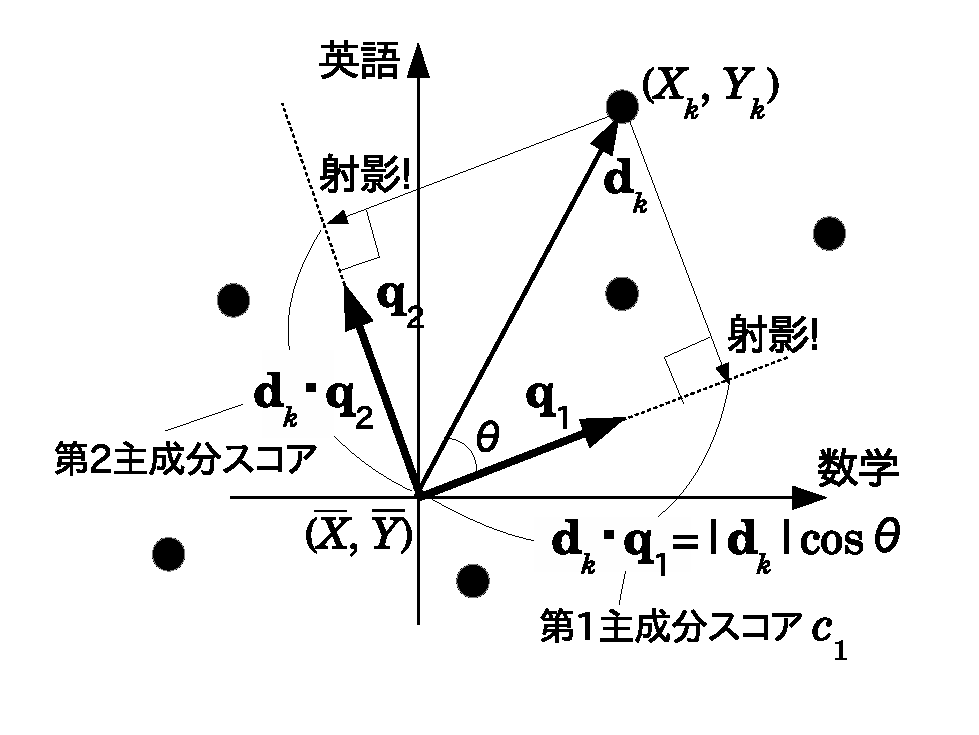
\includegraphics[width=8cm]{PCA_shaei.eps}
    \caption{中心化されたデータベクトル${\bf d}_k$を主成分ベクトルで分解する。
分解の係数(\eref{eq:PCA_lincomp}の$c_1, c_2$など)は, ${\bf d}_k$と主成分ベクトル
(${\bf q}_1$, ${\bf q}_2$など)との内積で得られる。それが各主成分スコアである。
それは, ${\bf d}_k$を主成分ベクトルに正射影(垂直に下ろすこと)したものでもある
(内積の定義から, ${\bf d}_k\bullet{\bf q}_1=|{\bf d}_k||{\bf q}_1|\cos\theta$。
$\theta$はこれらの2つのベクトルのなす角。いま, $|{\bf q}_1|=1$であることに注意すれば, 
これが正射影になっていることは明らかだろう)。\label{fig:PCA_shaei}}
\end{figure}


\begin{q}\label{q:PCA_006} 問\ref{q:PCA_001}の生徒3の得点の第1主成分スコア
と第2主成分スコアを求めよ。\end{q}

上の例では, 第1主成分スコアを数学と英語の両方を加味した総合成績
の指標と解釈すると, 第2主成分スコアは, 「数学と英語のどちらが得意か」
(あえて言えば, 理系向きか文系向きか)に関する指標と解釈することができる。

\begin{q}\label{q:PCA_008} 問\ref{q:PCA_001}の生徒3は理系向きか, 文系向きか, 考察せよ。\end{q}

{\small 注: 世間では, 「主成分」という言葉が単体で使われることがある。そのような
場合は, 「主成分」は, 以下のいずれかの意味を指す:
\begin{itemize}
\item 主成分ベクトル (ローディングベクトル)
\item 主成分スコア
\item 物質を構成する化学的な組成のうち, 最も大量に含まれるもの。
\end{itemize}
これらは互いに意味が違うので, どれを指すのかを, 文脈から適切に
判断しなければならない。そのような混乱を避けるために, 諸君は, 
「主成分」という言葉を, できるだけ単体では使わないようにしよう。\\}

{\small 注: 第1主成分をPC1, 第2主成分をPC2, ...のように言うこともある。
例えば, 「第1主成分スコア」を「PC1スコア」と言ったり, 「第2主成分ベクトル」
を「PC2ベクトル」と言ったりする。\\}


さて, 主成分分析の意味やからくりを, 少し調べてみよう。
分散共分散行列$S$は, \eref{eq:covmatrix_S_StD}や
\eref{eq:covar_matrix_sample3D}のように, 
中心化されたデータ行列$D_{\text{c}}$から求められる。
簡単のため, ここでは項目数=2で考える (項目数3以上であっても議論の本質は同じ)。
\eref{eq:covmatrix_S_StD}を\eref{eq:tQsQ_diag}に代入してみよう。
すなわち$\,^{\text t}QSQ$は以下のようになる:
\begin{eqnarray}
\,^{\text t}Q\Bigl(\frac{1}{N}\,^{\text t}D_{\text{c}}D_{\text{c}}\Bigr)Q=
\begin{bmatrix}
\lambda_1 & 0\\
0         & \lambda_2\\
\end{bmatrix}
\label{eq:tQsQ_diag2}\end{eqnarray}
この左辺は, 以下のように変形できる: 
\begin{eqnarray}
\,^{\text t}Q\Bigl(\frac{1}{N}\,^{\text t}D_{\text{c}}D_{\text{c}}\Bigr)Q=
\frac{1}{N}(\,^{\text t}Q\,^{\text t}D_{\text{c}})(D_{\text{c}}Q)\label{eq:tQsQ_diag2_30}\\
=\frac{1}{N}\,^{\text t}(D_{\text{c}}Q)(D_{\text{c}}Q)\label{eq:tQsQ_diag2_4}\end{eqnarray}
\eref{eq:tQsQ_diag2_30}から\eref{eq:tQsQ_diag2_4}への変形は\eref{eq:matrix_trans_prod02}
を使った。ここで, $D_{\text{c}}Q$という行列を改めて$D_{\text{c}}'$と置こう。つまり, 
\begin{eqnarray}
D_{\text{c}}':=D_{\text{c}}Q
\end{eqnarray}
とする。すると, \eref{eq:tQsQ_diag2_4}はさらに以下のように変形できる: 
\begin{eqnarray}
\frac{1}{N}\,^{\text t}D_{\text{c}}'D_{\text{c}}'
\label{eq:tQsQ_diag6}\end{eqnarray}
となる。これは, \eref{eq:covmatrix_S_StD}の右辺とよく
似ている。つまり, これは$D_{\text{c}}'$という行列が作る分散共分散行列である。

$D_{\text{c}}'$, つまり$D_{\text{c}}Q$という行列は, 
$D_{\text{c}}$に右から$Q$をかけたものである。
\eref{eq:AB_matprod_inprod}の考え方を使えば, $D_{\text{c}}Q$は$D_{\text{c}}$の
行ベクトルと, $Q$の列ベクトル (つまり$S$の主成分ベクトル)の内積で
作られる行列である。すなわち, 
\begin{eqnarray}
D_{\text{c}}'=D_{\text{c}}Q=\begin{bmatrix}
{\bf d}_1\bullet{\bf q}_1 & {\bf d}_1\bullet{\bf q}_2\\
{\bf d}_2\bullet{\bf q}_1 & {\bf d}_2\bullet{\bf q}_2\\
\vdots & \vdots\\
{\bf d}_N\bullet{\bf q}_1 & {\bf d}_N\bullet{\bf q}_2\\
\end{bmatrix}
\end{eqnarray}
となる。ここで, ${\bf d}_i$は$D_{\text{c}}$の第$i$行ベクトル(生徒$i$の得点を表す行ベクトル), 
${\bf q}_j$は$Q$の第$j$列ベクトル(第$j$主成分ベクトル)である。従って, ${\bf d}_i\bullet{\bf q}_j$は, 
生徒$i$の得点の第$j$主成分スコアに相当する。つまり, $D_{\text{c}}'$は, 各生徒の主成分スコアを並べた
行列である。$D_{\text{c}}'$は, 生徒全体の成績を表す, $D_{\text{c}}$とは別の新しい表現法である。
$D_{\text{c}}$は各科目の得点を(中心化して)並べたものだが, $D_{\text{c}}'$は各主成分のスコアを並べたものである。

例えば, 問\ref{q:PCA_004}の$Q, D_{\text{c}}$について, $D_{\text{c}}'=D_{\text{c}}Q$は以下の行列になる:
\begin{eqnarray}D_{\text{c}}'=D_{\text{c}}Q=\begin{bmatrix}
0.33\cdots  & -0.90\cdots\\
0.29\cdots  & 0.51\cdots\\
-2.54\cdots  & 0.42\cdots\\
-0.40\cdots  & -0.22\cdots\\
1.70\cdots  & 0.56\cdots\\
2.43\cdots  & -0.12\cdots\\
-1.81\cdots  & -0.26\cdots\\
\end{bmatrix}点\label{eq:PCA_001_DQ}\end{eqnarray}

この「新しい表現法」には, 面白い特徴がある: 
\eref{eq:tQsQ_diag2}, \eref{eq:tQsQ_diag6}より, 
\begin{eqnarray}
\frac{1}{N}\,^{\text t}D_{\text{c}}'D_{\text{c}}'=
\begin{bmatrix}
\lambda_1 & 0\\
0         & \lambda_2\\
\end{bmatrix}
\label{eq:tQsQ_diag8}\end{eqnarray}
である。つまり, この表現法では, 分散共分散行列が対角行列になるのだ。
これは, 主成分スコアどうしの共分散が0ということだ(分散共分散行列の
非対角成分が共分散を表すから。わからない人は, 
\eref{eq:def_covariance_matrix_sample}を見直すべし)。共分散が0になるなら, 
\eref{eq_def_sample_correlation}より, 相関係数も0である。すなわち, 
主成分スコアどうしは互いに連動しない。というよりも, そうなるような操作が
主成分分析なのである。テストの得点は, あるていど科目間で連動するだろう。
それを整理して, 互いに連動していない(いわば互いに「独立」な)指標
を作るのが主成分分析なのである。

先ほどの例で言えば, 第1主成分スコアが全体的な成績の良さ, 
第2主成分スコアが理系的か文系的かを表すと考えると, 意図的に
これらの間の連動性を消して(相関係数を0にして), それぞれを
独立・純粋に評価しようというのが, 主成分分析の発想である。

図\ref{fig:PCA_plot1}に, もとの行列$D_{\text{c}}$で表される成績
(数学と英語の各得点から平均点を引いたもの)の散布図, 
図\ref{fig:PCA_plot2}に, 行列$D_{\text{c}}'$で表される成績
(第1, 第2主成分スコア)の散布図を示す。これを見ると, 
もとの得点の散布図では, 数学の点が良ければ英語の点も
良い, というおおまかな傾向が見える。つまり, 両科目が
連動している。ところが, 主成分スコアの散布図を見ると, 
そのような連動する傾向は見えなくなっている。\\

このからくりは実は簡単である。すなわち, 図\ref{fig:PCA_plot1}
を, 原点を中心に右まわりに適当に回転させたら
図\ref{fig:PCA_plot2}になるのだ。逆に言えば, このような
連動が見られなくなるように, 散布図全体を回転するのが主成分
分析である。そして, $Q$はベクトルに回転を施す行列なのである。\\

また, 分散共分散行列の固有値は, 各主成分のスコアの分散に等しいことが, 
\eref{eq:tQsQ_diag8}からわかる。ところで, 分散共分散行列の
トレースを「全分散」\index{ぜんぶんさん@全分散}という。
問\ref{q:matrix_trace_PAP}より, それは分散共分散行列の固有値
(各主成分スコアの分散)の総和である。
先の例で言うと, 数学の分散と英語の分散の和は, 第1主成分スコアの分散と, 
第2主成分スコアの分散の和に等しい。

分散共分散行列の$i$番目の固有値, すなわち, 第$i$主成分のスコアの
分散を全分散で割ったものを\underline{第$i$主成分の寄与率}
\index{きよりつ@寄与率}という。\\

\begin{q}\label{q:PCA_012} 問\ref{q:PCA_004}において, 
第1主成分の寄与率と, 第2主成分の寄与率を求めよ。そこから
どういうことが言えるか考察せよ。\end{q}

\begin{figure}
    \centering
    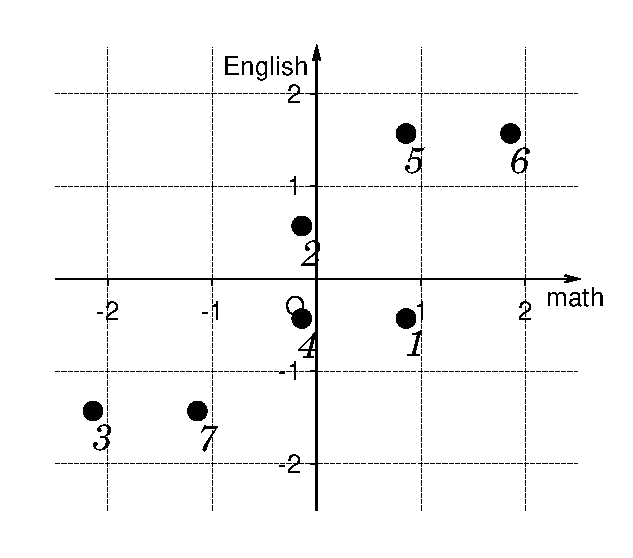
\includegraphics[width=6cm]{PCA_plot1.eps}
    \caption{\eref{eq:PCA_001_D}の散布図。各科目の得点から
平均点(標本平均)を引いた点数のプロット。番号は受験者の通し番号$k$。\label{fig:PCA_plot1}}
\end{figure}

\begin{figure}
    \centering
    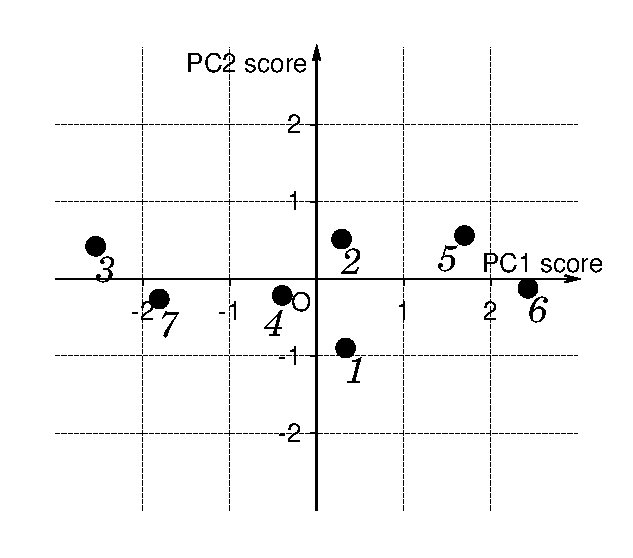
\includegraphics[width=6cm]{PCA_plot2.eps}
    \caption{\eref{eq:PCA_001_DQ}の散布図。第1主成分スコアを横軸, 
第2主成分スコアを縦軸とするプロット。番号は図\ref{fig:PCA_plot1}に対応する。\label{fig:PCA_plot2}}
\end{figure}

その他, まだまだ主成分分析にはいろんな用語や考え方がある。それらについては, 
「数理科学演習」で実例とともに学んで欲しい。いずれにせよ, 
対称行列の理論をきちんと理解すれば主成分分析は簡単であり, 
そういう理解の方が正しく主成分分析を使えるし, 応用も効くのだ。

\begin{faq}{\small\textgt{なぜ世の中には対称行列が多いのですか?}
 ... いくつかのものどうしの関係性を表すのに対称行列が適しているからです。
例えば, 分散共分散行列は, ざっくり言えば, 数学と英語という2種類の成績
が, 互いにどのように関係しているかを表すものと言えます。関係というものは
多くの場合, 対称的です。実際, 「数学と英語の関係」は「英語と数学の関係」
と言い換えても差し支えないでしょう。}\end{faq}
\mv


\section{数ベクトルの視覚表現}

これまで見たように, 多変量解析では, 個々のデータを数ベクトルとして
扱う。例えば, 数学, 英語, 国語という3科目からなる試験を実施した結果は, 
受験者それぞれについて, 各科目の得点を並べた数ベクトルが, データ
となる(多くの場合はそれを中心化して扱うのだが, ここではとりあえず
中心化は考えない)。例えば, 生徒A君の得点が, 数学: 10点, 英語: 20点, 
国語: 25点だとしたら, (10点, 20点, 25点)という数ベクトルが, A君に
関するデータである。

さて, 諸君は, この数ベクトルを視覚的にイメージせよと言われたらどうするだろう?
おそらく, 3次元空間をイメージし, 各科目の得点を, 互いに直交する軸にとって, 
数ベクトルが座標となるような空間中の1点もしくは, そこへ向う矢印を
イメージするだろう(図\ref{fig:vect_visual2}上)。
\begin{figure}
    \centering
    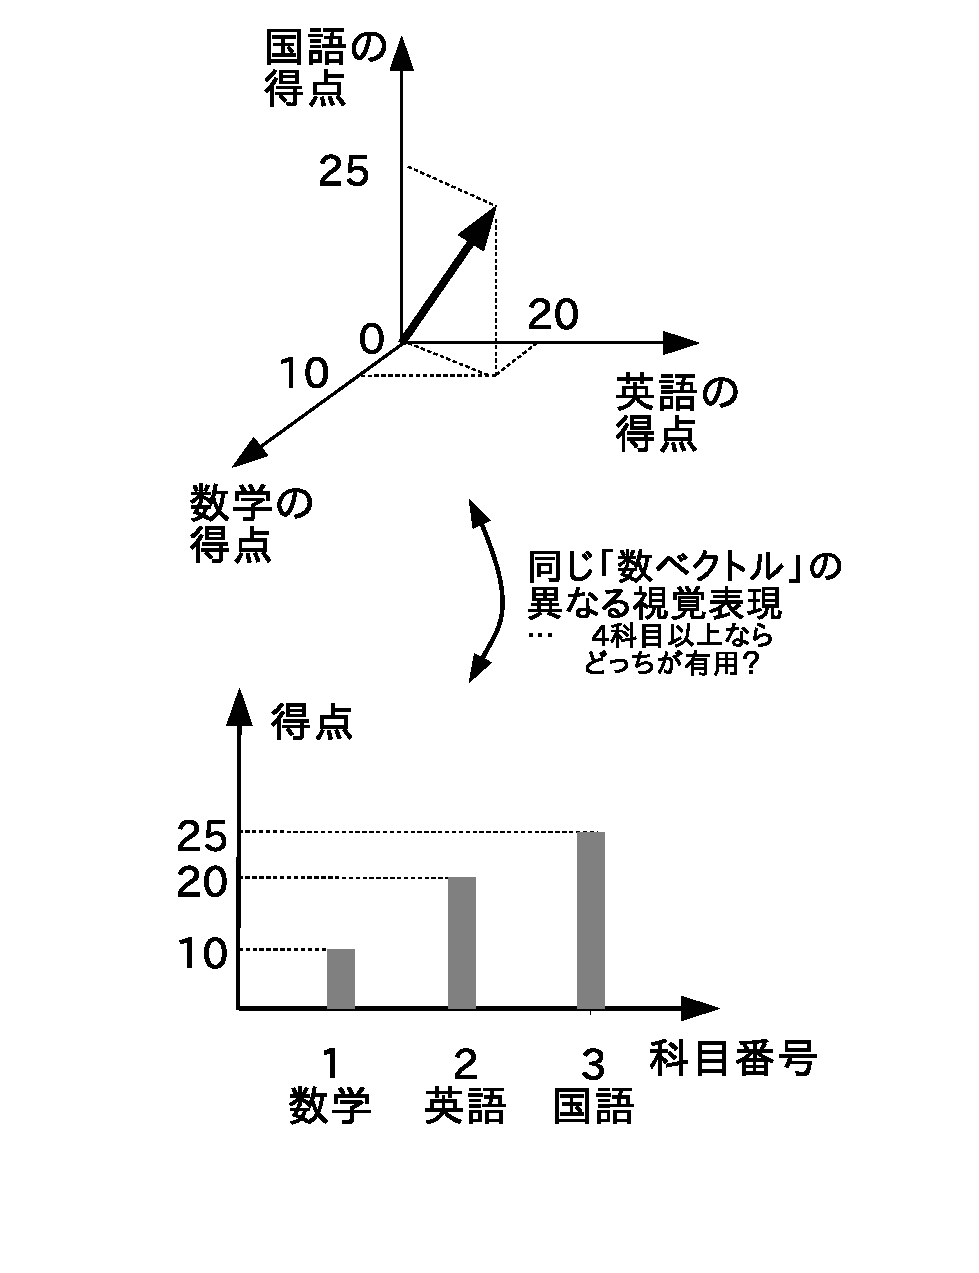
\includegraphics[width=8cm]{vect_visual2.eps}
    \caption{生徒A君の「成績ベクトル」の視覚表現(2通り)\label{fig:vect_visual2}}
\end{figure}

一方, これは, 図\ref{fig:vect_visual2}下のように, 各科目を横にならべて, 
棒グラフで表すこともできる。これら2つの表現方法は違うが, 表される「数ベクトル」
は同じものである。どちらの表現が正しいというものでもない。そもそも数ベクトルは
数を並べたものにすぎないのだから。

ところが, 試験の科目数が4以上になるとどうだろう? 明らかに, 上の表現(矢印)
は破綻する。人間は, 視覚的にイメージできるのは3次元までだからだ。
しかし下の表現(グラフ)は, 全く問題なく通用する。横に項目を
増やしていけばよいだけだ。

そう考えると, 諸君が高校時代から「ベクトル」について素朴に抱いていた「矢印」
のイメージ(図\ref{fig:vect_visual2}上)は, 実は数ベクトルの実体を表す
には不便だと気づくだろう。むしろ, 図\ref{fig:vect_visual2}下のような, 
「グラフ」の方が, ベクトルのイメージとしては柔軟ではないか? 

\begin{q}\label{q:vect_image2} 数ベクトルを矢印ではなくグラフでイメージ
することについて, 君自身はどう感じるか?\end{q}

\begin{faq}{\small\textgt{数学がこれほど密に統計や化学と結びついてる
とは知りませんでした}... まだまだ, こんなもんじゃありません。}\end{faq}


\section{解答}

% 3つの行列$A, B, C$を考える。
%\noindent{\textbf{答}}\ref{q:invmatrix_product3} 略。\\

% $n$次正則行列$A, B$について, 
\noindent{\textbf{答}}\ref{q:invmatrix_product} (略解) $AB$の右から$B^{-1}A^{-1}$をかけると, 
\begin{eqnarray}
(AB)(B^{-1}A^{-1})=A\{B(B^{-1}A^{-1})\}\label{q:invmatrix_product_2}
\end{eqnarray}
となる。ここで\eref{eq:matrix_association_law}を使った(\eref{eq:matrix_association_law}の
$C$を$B^{-1}A^{-1}$とした)。この右辺の$\{\}$内に再び\eref{eq:matrix_association_law}を
使うと(\eref{eq:matrix_association_law}を右辺から左辺に向けて使う。\eref{eq:matrix_association_law}
の$A$を$B$とし, \eref{eq:matrix_association_law}の$B$を$B^{-1}$, $C$を$A^{-1}$とする), 
\eref{q:invmatrix_product_2}の右辺は, 
\begin{eqnarray}
A\{B(B^{-1}A^{-1})\}=A\{(BB^{-1})A^{-1}\}\label{q:invmatrix_product_4}
\end{eqnarray}
となる。逆行列の定義から, $BB^{-1}=I$なので, \eref{q:invmatrix_product_4}の右辺は, 
\begin{eqnarray}
A\{(BB^{-1})A^{-1}\}=A(IA^{-1})=AA^{-1}=I\label{q:invmatrix_product_6}
\end{eqnarray}
となる。\eref{q:invmatrix_product_2}, \eref{q:invmatrix_product_4}, \eref{q:invmatrix_product_6}
より, 
\begin{eqnarray}
(AB)(B^{-1}A^{-1})=I\label{q:invmatrix_product_8}
\end{eqnarray}
が成り立つ。同様に, $AB$の左から$B^{-1}A^{-1}$をかけると(...中略...), 
\begin{eqnarray}
(B^{-1}A^{-1})(AB)=I\label{q:invmatrix_product_9}
\end{eqnarray}
が成り立つ。\eref{q:invmatrix_product_8}, \eref{q:invmatrix_product_9}と, 
逆行列の定義より, $B^{-1}A^{-1}$は$(AB)$の逆行列である。すなわち\eref{eq:ABinverse}が成り立つ。\\

% 2つの3次元列ベクトル(3行1列の行列)
\noindent{\textbf{答}}\ref{q:linear2_40} 
\begin{edaenumerate}
\item $ax+by+cz$
\item $ax+by+cz$
\item 
\begin{eqnarray*}
\begin{bmatrix}
ax  &  ay &  az\\
bx  &  by &  bz\\
cx  &  cy &  cz\\
\end{bmatrix}
\end{eqnarray*}
\item 
\begin{eqnarray*}
\begin{bmatrix}
ax  &  bx &  cx\\
ay  &  by &  cy\\
az  &  bz &  cz\\
\end{bmatrix}
\end{eqnarray*}
\end{edaenumerate}
\vspace{0.2cm}

% 実数を成分とする, 任意の
%\noindent{\textbf{答}}\ref{q:transpose_inprod} 略(行列の積の定義から導く。簡単!)。\\

% \eref{eq:exmpl_matrix_A00}の$A$と
%\noindent{\textbf{答}}\ref{q:tAx_txtA_exmpl} 略。\\

%\noindent{\textbf{答}}\ref{q:tAB_tBtA_proof} 略。\\

% $n$次正方行列$A, B$について, 次式を示せ:
\noindent{\textbf{答}}\ref{q:matrix_trace} \\
\begin{enumerate}
\item
\begin{eqnarray*}
\tr(A+B)=\sum_{i} [A+B]_{ii}=\sum_{i}([A]_{ii}+[B]_{ii})\\
=\sum_{i}[A]_{ii}+\sum_{i}[B]_{ii}=\tr(A)+\tr(B)
\end{eqnarray*}
\item
\begin{eqnarray*}
\tr(AB)&=&\sum_{i}[AB]_{ii}\\
&=&\sum_{i}\sum_{k}[A]_{ik}[B]_{ki}\\
&=&\sum_{i}\sum_{k}[B]_{ki}[A]_{ik}\\
&=&\sum_{k}\sum_{i}[B]_{ki}[A]_{ik}\\
&=&\sum_{k}[BA]_{kk}=\tr(BA)
\end{eqnarray*}
\item
\begin{eqnarray*}
\tr(^{\text t}A)&=&\sum_{i}[^{\text t}A]_{ii}=\sum_{i}[A]_{ii}=\tr(A)
\end{eqnarray*}
\end{enumerate}
\vv

% $A$を任意の行列とする(正方行
\noindent{\textbf{答}}\ref{q:matrix_symmetry_exmpl1} \\
(1) \eref{eq:matrix_trans_prod02}より, 
\begin{eqnarray}
^{\text t}(^{\text t}AA)=\,^{\text t}A\,^{\text t}(^{\text t}A)\label{eq:matrix_symmetry_exmpl1}
\end{eqnarray}
また, $^{\text t}(^{\text t}A)=A$だから, \eref{eq:matrix_symmetry_exmpl1}右辺は, $^{\text t}AA$となる。
従って, $^{\text t}(^{\text t}AA)=\,^{\text t}AA$となる。すなわち, $^{\text t}AA$は対称行列。
(2)は略。\\

%\noindent{\textbf{答}}\ref{q:A_tA_2_symmetry} 略(簡単!)。\\

\noindent{\textbf{答}}\ref{q:covar_matrix} 
{\small
\begin{eqnarray}
&&\,^{\text t}D_{\text{c}}D_{\text{c}}=\nonumber\\
&&\begin{bmatrix}
X_1 - \overline{X} & X_2 - \overline{X} & \cdots & X_N - \overline{X}\\
Y_1 - \overline{Y} & Y_2 - \overline{Y} & \cdots & Y_N - \overline{Y}\\
\end{bmatrix}
\begin{bmatrix}
X_1 - \overline{X} & Y_1 - \overline{Y}\\
X_2 - \overline{X} & Y_2 - \overline{Y}\\
\vdots             & \vdots\\
X_N - \overline{X} & Y_N - \overline{Y}\\
\end{bmatrix}\nonumber\\
&&=
\begin{bmatrix}
(X_1 - \overline{X})^2+\cdots & (X_1 - \overline{X})(Y_1-\overline{Y})+\cdots\\
(X_1 - \overline{X})(Y_1-\overline{Y})+\cdots & (Y_1 - \overline{Y})^2+\cdots\\
\end{bmatrix}\nonumber\\
&&=
\begin{bmatrix}
\sum_{k=1}^N (X_k-\overline{X})^2 & \sum_{k=1}^N (X_k-\overline{X})(Y_k-\overline{Y})\\
\sum_{k=1}^N (X_k-\overline{X})(Y_k-\overline{Y}) & \sum_{k=1}^N (Y_k-\overline{Y})^2\\
\end{bmatrix}\nonumber\\
\end{eqnarray}}
これを$N$で割ると, \eref{eq:def_s2X}, \eref{eq:def_s2Y}, \eref{eq:def_sXY}より, 
\begin{eqnarray}
\left[\begin{array}{ccc}
s_{X}^2 & s_{XY}\\
s_{XY}  & s_{Y}^2\\
\end{array}\right]=S
\end{eqnarray}
となる。\\

\noindent{\textbf{答}}\ref{q:PCA_001} 以下, 数値は小数点
以下2桁まで書くが, 諸君はレポートでは小数点以下4桁までを書くこと(それを自力で計算した証拠とみなす)。
\begin{enumerate}
\item $\overline{X}=3.14\cdots$点, $\overline{Y}=3.42\dots$点
\item 略。
\item 
\begin{eqnarray*}S=\frac{1}{7}\,^{\text t}D_{\text{c}}D_{\text{c}}=
\begin{bmatrix}
1.55\cdots & 1.22\cdots\\
1.22\cdots & 1.38\cdots\\
\end{bmatrix}\text{点}^2\end{eqnarray*}
\item 前小問より, $s_{X}^2=1.55\cdots$点$^2$, \\$s_{Y}^2=1.38\cdots$点$^2$, $s_{XY}=1.22\cdots$点$^2$。 
\item $s_{XY}/(s_{X}s_{Y})=1.22\cdots/\sqrt{1.55\cdots\times1.38\cdots}=0.83\cdots$。
\end{enumerate}
ちなみに, この問題を, 統計解析ソフトRを使ってやる方法(コマンド)を以下に示す:\\
 mth $<$-c(4,3,1,3,4,5,2)\\
(↑数学得点を並べた数ベクトルをmthと定義)\\
 eng $<$-c(3,4,2,3,5,5,2)\\
(↑英語得点を並べた数ベクトルをengと定義)\\
 mean(mth)\\
(↑数学の標本平均)\\
 mean(eng)\\
(↑英語の標本平均)\\
 Dc=cbind(mth-mean(mth),eng-mean(eng))\\
(↑行列$D_{\text{c}}$を定義。)\\
 Dc\\
(↑行列$D_{\text{c}}$の成分を表示)\\
 S=t(Dc)\%*\%Dc/7.0\\
(↑\eref{eq:covmatrix_S_StD}を計算)\\
 S\\
(↑行列$S$の成分を表示)\\
 S[1,2]/(sqrt(S[1,1]*S[2,2]))\\
(↑\eref{eq_def_sample_correlation}を計算)\\
 cor(mth,eng)\\
(↑念の為, Rの標準関数を使って相関係数を計算。上の計算と合っていることを確認)\\

\noindent{\textbf{答}}\ref{q:matrix_orthogonal_exmpl1} 略 (いずれも
\eref{eq:def_orthogmatrix02}が成り立つことを計算で確かめればよい)。\\

\noindent{\textbf{答}}\ref{q:AB_orthogmatrix} 直交行列
\begin{eqnarray*}
Q=\begin{bmatrix}
q_{11} & q_{12} & \cdots & q_{1n}\\
q_{21} & q_{22} & \cdots & q_{2n}\\
\vdots & \vdots & \ddots & \vdots\\
q_{n1} & q_{n2} & \cdots & q_{nn}\\
\end{bmatrix}
\end{eqnarray*}
の第$i$列ベクトルを, ${\bf q}_i$とする。すなわち, 
\begin{eqnarray*}
{\bf q}_i=\begin{bmatrix}
q_{1i}\\
q_{2i}\\
\vdots\\
q_{ni}\\
\end{bmatrix}
\end{eqnarray*}
とする。すると, 
\begin{eqnarray}
^{\text t}Q\,Q&=&
\begin{bmatrix}
q_{11} & q_{21} & \cdots & q_{n1}\\
q_{12} & q_{22} & \cdots & q_{n2}\\
\vdots & \vdots & \ddots & \vdots\\
q_{1n} & q_{2n} & \cdots & q_{nn}\\
\end{bmatrix}
\begin{bmatrix}
q_{11} & q_{12} & \cdots & q_{1n}\\
q_{21} & q_{22} & \cdots & q_{2n}\\
\vdots & \vdots & \ddots & \vdots\\
q_{n1} & q_{n2} & \cdots & q_{nn}\\
\end{bmatrix}\nonumber\\
&=&
\begin{bmatrix}
{\bf q}_1\bullet{\bf q}_1 & {\bf q}_1\bullet{\bf q}_2 & \cdots & {\bf q}_1\bullet{\bf q}_n\\
{\bf q}_2\bullet{\bf q}_1 & {\bf q}_2\bullet{\bf q}_2 & \cdots & {\bf q}_2\bullet{\bf q}_n\\
\vdots & \vdots & \ddots & \vdots\\
{\bf q}_n\bullet{\bf q}_1 & {\bf q}_n\bullet{\bf q}_2 & \cdots & {\bf q}_n\bullet{\bf q}_n\\
\end{bmatrix}\label{eq:AB_orthogmatrix_ans4}
\end{eqnarray}
となる。積の$(i, j)$成分は$^{\text t}Q$の第$i$行ベクトル
と$Q$の第$j$列ベクトル${\bf q}_j$の内積であり, なおかつ, $^{\text t}Q$の第$i$行ベクトルは
$Q$の第$i$列ベクトル${\bf q}_i$の転置ベクトルであることから, 積の$(i, j)$成分は
${\bf q}_i\bullet{\bf q}_j$であることを使った。一方, $Q$は直交行列なので, 直交行列の定義から, 
\begin{eqnarray}
^{\text t}Q\,Q=I=
\begin{bmatrix}
1 & 0 & \cdots & 0\\
0 & 1 & \cdots & 0\\
\vdots & \vdots & \ddots & \vdots\\
0 & 0 & \cdots & 1\\
\end{bmatrix}\label{eq:AB_orthogmatrix_ans6}
\end{eqnarray}
となるはず。\eref{eq:AB_orthogmatrix_ans4}と\eref{eq:AB_orthogmatrix_ans6}を比べる。
対角成分どうしの比較から, 
\begin{eqnarray*}
{\bf q}_i\bullet{\bf q}_i=|{\bf q}_i|^2=1
\end{eqnarray*}
が成り立つ。すなわち$|{\bf q}_i|=1$, すなわち$Q$の列ベクトルは大きさが1である。
また, 非対角成分どうしの比較から, 
\begin{eqnarray*}
{\bf q}_i\bullet{\bf q}_j=0
\end{eqnarray*}
である ($i\neq j$とする)。すなわち, $Q$の列ベクトルどうしは互いに直交する。\qed
\mv

%
\noindent{\textbf{答}}\ref{q:orthonorm_vec_ortogonal_matrix} 互いに直交し, それぞれの
大きさが1であるような$n$次元の列ベクトル$n$個が, ${\bf p}_1, {\bf p}_2, \cdots, {\bf p}_n$
であるとする。これらを横に並べてできる$n$次正方行列$P$は, 
\begin{eqnarray}P=
\begin{bmatrix}
          &           &         &         \\
{\bf p}_1 & {\bf p}_2 & \cdots & {\bf p}_n\\
          &           &        &          \\
\end{bmatrix}
\end{eqnarray}
となる。従って, その転置行列$^{\text t}P$は以下のようになる。
\begin{eqnarray}^{\text t}P=
\begin{bmatrix}
 &  & ^{\text t}{\bf p}_1 &  & \\
 &  & ^{\text t}{\bf p}_2 &  & \\
 &  & \vdots &  & \\
 &  & ^{\text t}{\bf p}_n &  & \\
\end{bmatrix}
\end{eqnarray}
($^{\text t}{\bf p}_1$等は$n$次の行ベクトルであることに注意)。従って, 
\begin{eqnarray}
&&^{\text t}PP=
\begin{bmatrix}
 &  & ^{\text t}{\bf p}_1 &  & \\
 &  & ^{\text t}{\bf p}_2 &  & \\
 &  & \vdots &  & \\
 &  & ^{\text t}{\bf p}_n &  & \\
\end{bmatrix}
\begin{bmatrix}
          &           &         &         \\
{\bf p}_1 & {\bf p}_2 & \cdots & {\bf p}_n\\
          &           &        &          \\
\end{bmatrix}\nonumber\\
&&=\begin{bmatrix}
{\bf p}_1\bullet{\bf p}_1 & {\bf p}_1\bullet{\bf p}_2 & \cdots & {\bf p}_1\bullet{\bf p}_n\\
{\bf p}_2\bullet{\bf p}_1 & {\bf p}_2\bullet{\bf p}_2 & \cdots & {\bf p}_2\bullet{\bf p}_n\\
\vdots & \vdots & \ddots & \vdots\\
{\bf p}_n\bullet{\bf p}_1 & {\bf p}_n\bullet{\bf p}_2 & \cdots & {\bf p}_n\bullet{\bf p}_n\\
\end{bmatrix}\label{eq:orthonorm_vec_ortogonal_matrix_ans5}
\end{eqnarray}
となる。ここで, 任意の$i$について${\bf p}_i\bullet{\bf p}_i=1$であり(大きさが1だから!), 
任意の$i, j$ ($i\neq j$とする)について${\bf p}_i\bullet{\bf p}_j=0$である(互いに直交するから!)
ことから, \eref{eq:orthonorm_vec_ortogonal_matrix_ans5}の最終項は, 対角成分が1, 非対角成分が0
の正方行列, つまり単位行列になる。つまり, $^{\text t}PP=I$となる。従って, $P$は直交行列。\qed
\mv

\noindent{\textbf{答}}\ref{q:orthonorm_vec_ortogonal_matrix2} 略解: $Q$を$n$次の直交行列として, 
\begin{eqnarray}Q=
\begin{bmatrix}
          &           &         &         \\
{\bf q}_1 & {\bf q}_2 & \cdots & {\bf q}_n\\
          &           &        &          \\
\end{bmatrix}
\end{eqnarray}
と置く(${\bf q}_1$, ${\bf q}_2$, ...は$Q$を構成する列ベクトル)。\eref{eq:orthonorm_vec_ortogonal_matrix_ans5}
と同様に考えて, 
\begin{eqnarray*}
^{\text t}QQ
=\begin{bmatrix}
{\bf q}_1\bullet{\bf q}_1 & {\bf q}_1\bullet{\bf q}_2 & \cdots & {\bf q}_1\bullet{\bf q}_n\\
{\bf q}_2\bullet{\bf q}_1 & {\bf q}_2\bullet{\bf q}_2 & \cdots & {\bf q}_2\bullet{\bf q}_n\\
\vdots & \vdots & \ddots & \vdots\\
{\bf q}_n\bullet{\bf q}_1 & {\bf q}_n\bullet{\bf q}_2 & \cdots & {\bf q}_n\bullet{\bf q}_n\\
\end{bmatrix}
\end{eqnarray*}
$Q$は直交行列なのだから, これは単位行列に等しい, つまり対角成分は1で非対角成分は0になる。
対角成分は, $Q$の各列ベクトルの大きさの2乗であり, それが1に等しいことから, $Q$の
各列ベクトルの大きさは1である。また, 非対角成分は, $Q$の列ベクトルどうしの内積であり, 
それらが0であることから, $Q$の列ベクトルどうしは直交する。\qed
\mv
%
%\noindent{\textbf{答}}\ref{q:symmmetry_matrix_eigenvec_ort} 略。ヒントに従って考えよう!\\
%
%\noindent{\textbf{答}}\ref{q:symmmetry_matrix_eigenvec_ort_exmpl} 略。\\
%
\noindent{\textbf{答}}\ref{q:symmetry_matrix_diagonalize01} 以下, 略解。
レポートでは途中経過も記すこと。注: 固有ベクトルは大きさ1にすること。でないと
それを並べた時に直交行列にならない。
\begin{eqnarray*}
&&\text(1)\,\,\,Q=\begin{bmatrix}
2/\sqrt{5} & -1/\sqrt{5}\\
1/\sqrt{5} & 2/\sqrt{5}\\
\end{bmatrix}, \,\,\,
\,^{\text t}Q AQ=\begin{bmatrix}
3 & 0\\
0 & -2\\
\end{bmatrix}\\
&&\text(2)\,\,\,Q=\begin{bmatrix}
2/3 &  1/3 &  2/3\\
2/3 & -2/3 & -1/3\\
1/3 &  2/3 & -2/3\\
\end{bmatrix}, \,\,\,
\,^{\text t}Q AQ=\begin{bmatrix}
3 & 0 & 0\\
0 & 0 & 0\\
0 & 0 & -3\\
\end{bmatrix}
\end{eqnarray*}
注: 上の各行列で, 各列ベクトルが$\pm$逆になっていてもOK。例えば(1)では
\begin{eqnarray*}
Q=\begin{bmatrix}
2/\sqrt{5} & 1/\sqrt{5}\\
1/\sqrt{5} & -2/\sqrt{5}\\
\end{bmatrix}
\end{eqnarray*}
でもOK。\mv

\noindent{\textbf{答}}\ref{q:matrix_trace_PAP}
\eref{eq:matrix_trace_AB_BA}より, 
\begin{eqnarray*}
\tr(P^{-1}AP)&=&\tr(P^{-1}(AP))=\tr((AP)P^{-1})\\
&=&\tr(A(PP^{-1}))=\tr(AI)=\tr(A)
\end{eqnarray*}
従って, $\tr(A)$は, 対角化された行列$P^{-1}AP$のトレースに等しい。$P^{-1}AP$の
対角成分は$\lambda_1, \lambda_2, \cdots, \lambda_n$なので, 
$\tr(A)=\lambda_1+\lambda_2+\cdots+\lambda_n$。\qed
\mv

%
\noindent{\textbf{答}}\ref{q:PCA_004} (略解) 以下, 
数値は小数点以下2桁で書くが, 諸君はレポートでは小数点以下
4桁以上を書くこと(それを自力で計算した証拠とみなす)。
まず, 特性方程式を立てて解く(2次方程式の解の公式を使う)と, 
固有値は$\lambda_1=2.69\dots$, $\lambda_2=0.24\cdots$
と求まる。それを元に固有ベクトルを求めると, 
\begin{eqnarray}
{\bf q}_1=\begin{bmatrix}
0.73\cdots\\
0.68\cdots\\
\end{bmatrix},\,
{\bf q}_2=\begin{bmatrix}
-0.68\cdots\\
0.73\cdots\\
\end{bmatrix}\label{eq:PCA_004ans2}
\end{eqnarray}
となる。従って, 
\begin{eqnarray}
Q=\begin{bmatrix}
0.73\cdots & -0.68\cdots\\
0.68\cdots & 0.73\cdots\\
\end{bmatrix}\text{として, }\\
\,^{\text t}QSQ=\begin{bmatrix}
2.69\dots & 0\\
0 & 0.24\cdots\\
\end{bmatrix}\text{点}^2
\end{eqnarray}
注: 分散共分散行列の固有値は, 分散と同じ次元を持つ(この場合は点$^2$)と考え, 
固有ベクトルの成分は無次元と考えると都合が良い。従って, ここでは$\,^{\text t}QSQ$
に点$^2$という単位をつけ, 他の数値には単位をつけない。\\

%
\noindent{\textbf{答}}\ref{q:PCA_005} \eref{eq:PCA_004ans2}の
${\bf q}_1, {\bf q}_2$がそれぞれ第1主成分ベクトルと第2主成分ベクトル。\\

%
\noindent{\textbf{答}}\ref{q:PCA_005c} 生徒3の数学と英語の
得点はそれぞれ1点と2点。それぞれから数学の平均点と英語の平均点を
引いて並べると, $(-2.14, -1.42)$点となる(これは\eref{eq:PCA_001_D}の
第3行ベクトルである)。\\

%
\noindent{\textbf{答}}\ref{q:PCA_006} 問\ref{q:PCA_005c}より, 
生徒3の中心化されたデータベクトルは$(-2.14, -1.42)$点である。
この行ベクトルを${\bf d}$とする。\eref{eq:PCA_004ans2}の${\bf q}_1, {\bf q}_2$
を使って, 第1主成分スコア$={\bf d}\bullet{\bf q}_1=-2.54\cdots$, 
第2主成分スコア$={\bf d}\bullet{\bf q}_2=0.42\cdots$。\\

\noindent{\textbf{答}}\ref{q:PCA_008} 第2主成分スコアがプラスである, 
すなわち, 数学よりも英語の方ができるという傾向が見える。文系にも数学は
必要だし理系にも英語は必要なので一概には言えないが, どちらかと言えば
文系...?\\

\noindent{\textbf{答}}\ref{q:PCA_012} $\lambda_1=2.69$, $\lambda_2=0.24$, 
$\tr(S)=2.94$。従って, 第1主成分の寄与率=2.69/2.94=0.92。
第2主成分の寄与率=0.24/2.94=0.08。この結果を見ると, 第1主成分の寄与率が
圧倒的に大きい。つまり, この試験結果を数学と英語の2次元数ベクトルの集合
とみたときのばらつき(全分散)は, 両科目の総合的な成績(第1主成分スコア)のばらつき
が主たる要因であり, それは理系的か文系的かという適性(第2主成分スコア)
によるばらつきよりもずっと大きく寄与していると考えられる。
\mv

\noindent{\textbf{答}}\ref{q:vect_image2} 略。君自身の感じ方を述べよ。
「何も感じない」はダメ。
